% !TeX encoding = UTF-8
\chapter{Task 3: Comparison}\label{chap:task3}

All numbers in this chapter are on the 33,463 test flows (19,202 DDoS, 14,261 BENIGN) unless stated otherwise. DDoS is the positive class; a false positive (FP) is a benign flow flagged as an attack and a false negative (FN) is a missed attack.

\section{Comparison table}
Table~\ref{tab:main} lists Accuracy, Precision, Recall, F1 (the F-score) and ROC-AUC, together with the confusion counts and the cost of each model. The rows are sorted by F1. We omit the image version of this table (\texttt{comparison\_table}) because the table below contains the same numbers.

\begin{table}[htb]
\centering
\caption{Test results of all eight models, sorted by F1 (train and predict times in seconds).}\label{tab:main}
\footnotesize\setlength{\tabcolsep}{3pt}\resizebox{\textwidth}{!}{% booktabs table (4-decimal scores, 3-decimal times). Wide: wrap it in
% \resizebox{\textwidth}{!}{ ... } and \usepackage{booktabs}.
\begin{tabular}{lrrrrrrrrrrr}
\toprule
Model & Accuracy & Precision & Recall & F1 & ROC-AUC & TP & TN & FP & FN & Train (s) & Predict (s) \\
\midrule
XGBoost & 1.0000 & 1.0000 & 1.0000 & 1.0000 & 1.0000 & 19202 & 14261 & 0 & 0 & 2.021 & 0.017 \\
Random Forest & 0.9999 & 1.0000 & 0.9998 & 0.9999 & 1.0000 & 19199 & 14261 & 0 & 3 & 3.847 & 0.092 \\
K-Nearest Neighbors & 0.9998 & 0.9999 & 0.9997 & 0.9998 & 0.9999 & 19197 & 14260 & 1 & 5 & 0.008 & 4.204 \\
MLP & 0.9995 & 0.9997 & 0.9994 & 0.9995 & 1.0000 & 19190 & 14255 & 6 & 12 & 42.244 & 0.008 \\
LSTM & 0.9990 & 0.9992 & 0.9992 & 0.9992 & 1.0000 & 19186 & 14245 & 16 & 16 & 136.034 & 0.173 \\
1D-CNN & 0.9990 & 0.9993 & 0.9990 & 0.9991 & 1.0000 & 19182 & 14248 & 13 & 20 & 65.544 & 0.086 \\
Logistic Regression & 0.9980 & 0.9977 & 0.9988 & 0.9983 & 0.9999 & 19179 & 14217 & 44 & 23 & 17.348 & 0.001 \\
Gaussian Naive Bayes & 0.9895 & 0.9832 & 0.9986 & 0.9909 & 0.9880 & 19176 & 13934 & 327 & 26 & 0.063 & 0.010 \\
\bottomrule
\end{tabular}
}
\end{table}

Figure~\ref{fig:small} ranks the models per metric and Figure~\ref{fig:heat} shows all scores at once. With scores this close to 1, the axes of Figure~\ref{fig:small} are zoomed, so the bars exaggerate small differences; the numbers on the bars are the reliable information.

\begin{figure}[htb]
\centering
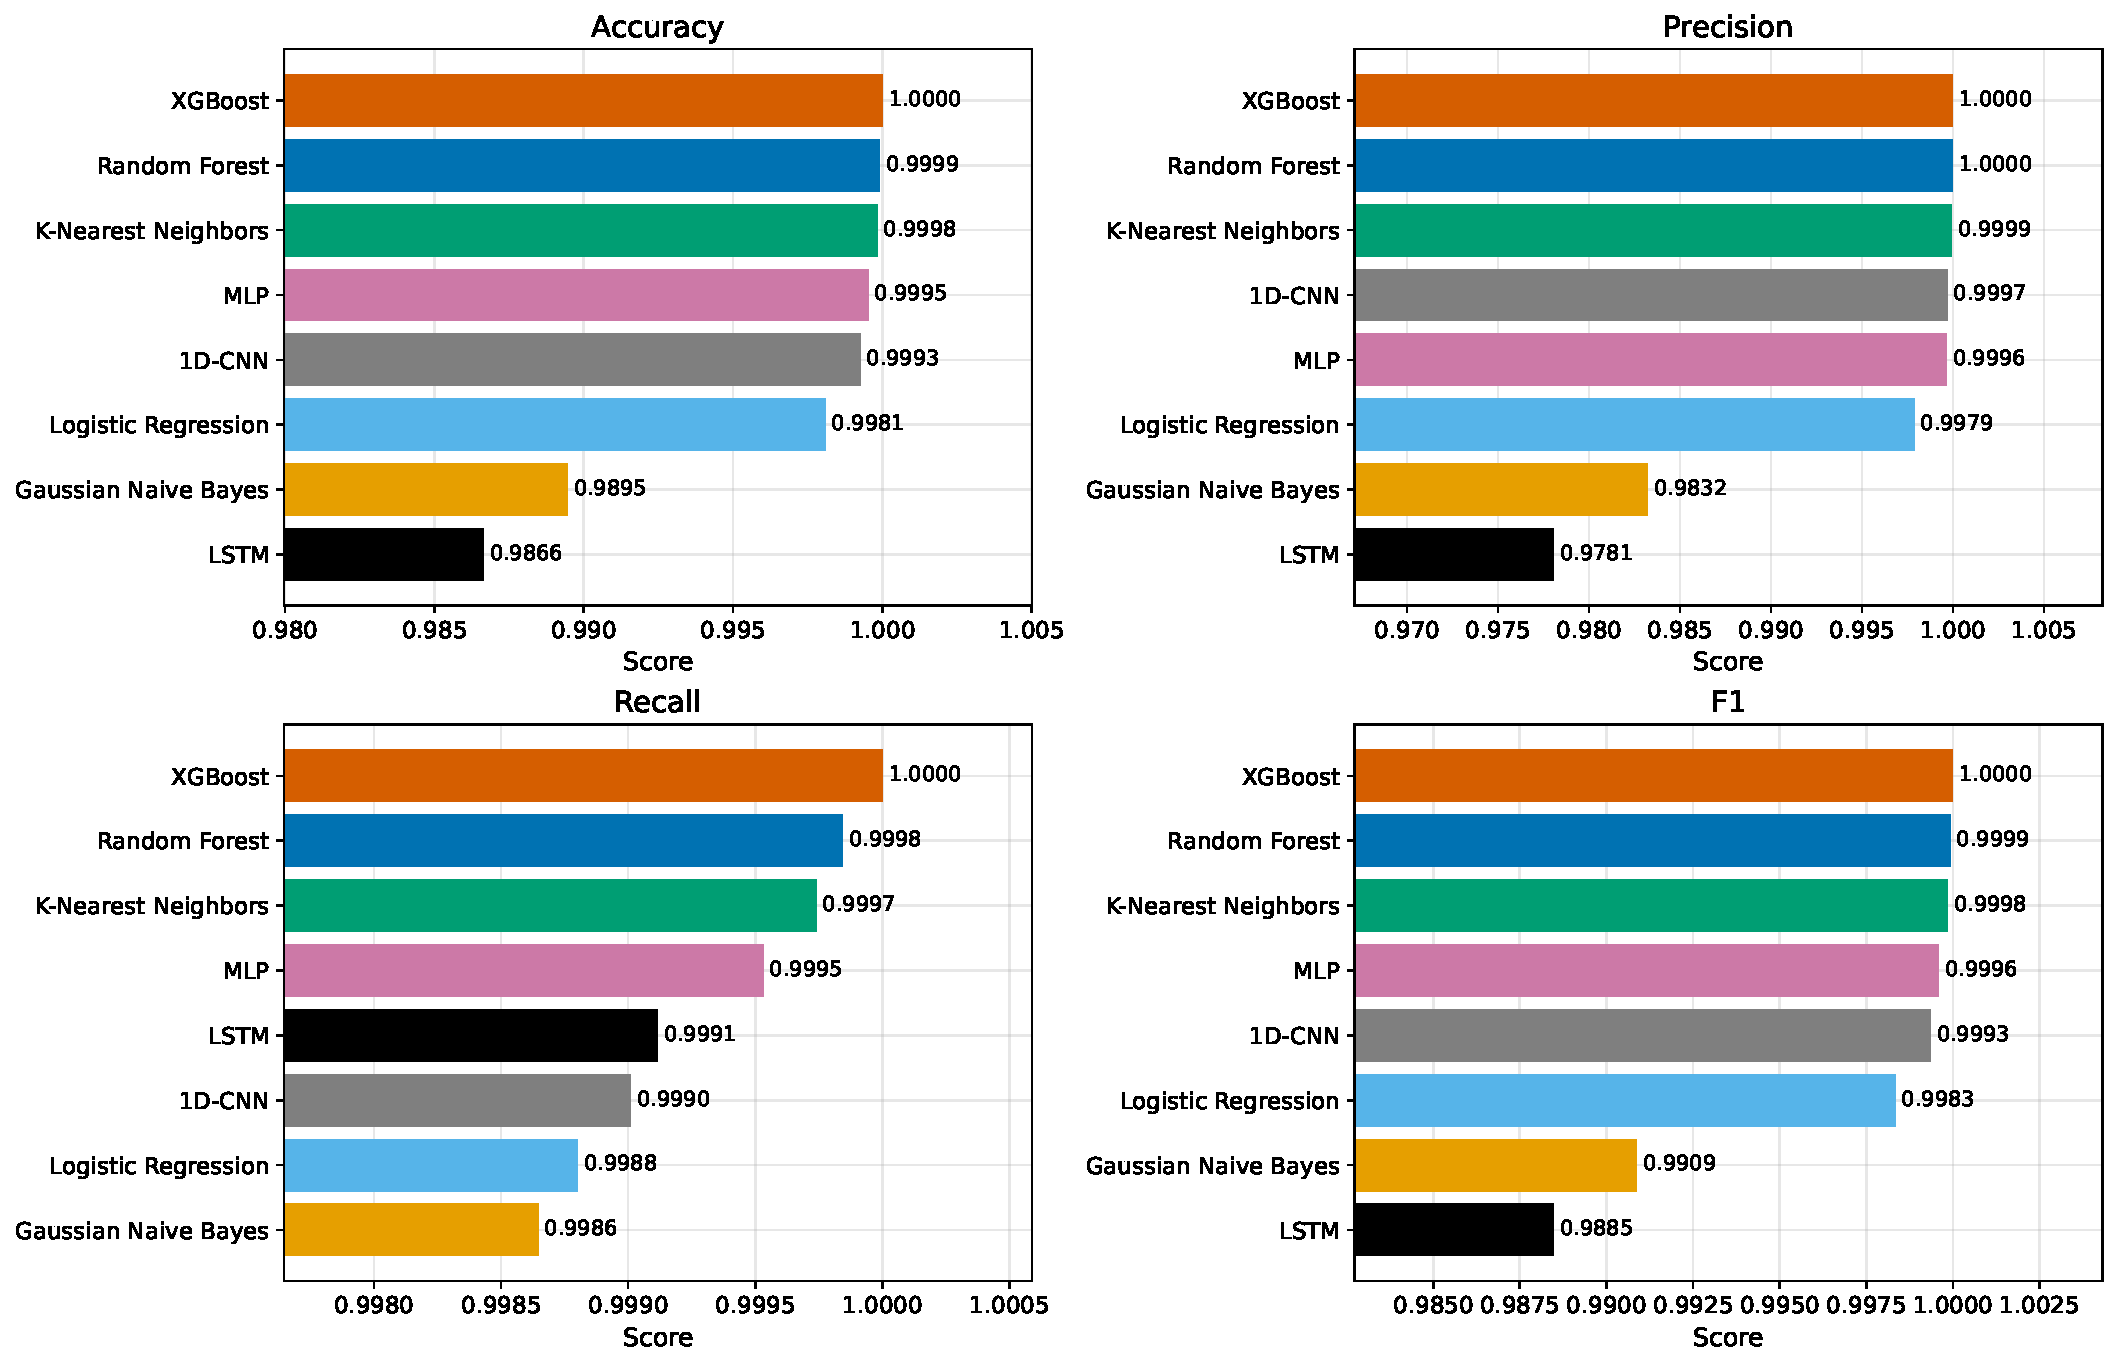
\includegraphics[width=0.9\textwidth]{metrics_small_multiples.pdf}
\caption{Accuracy, Precision, Recall and F1 of all models, one panel per metric, sorted by score. The axes are truncated.}\label{fig:small}
\end{figure}

\begin{figure}[htb]
\centering
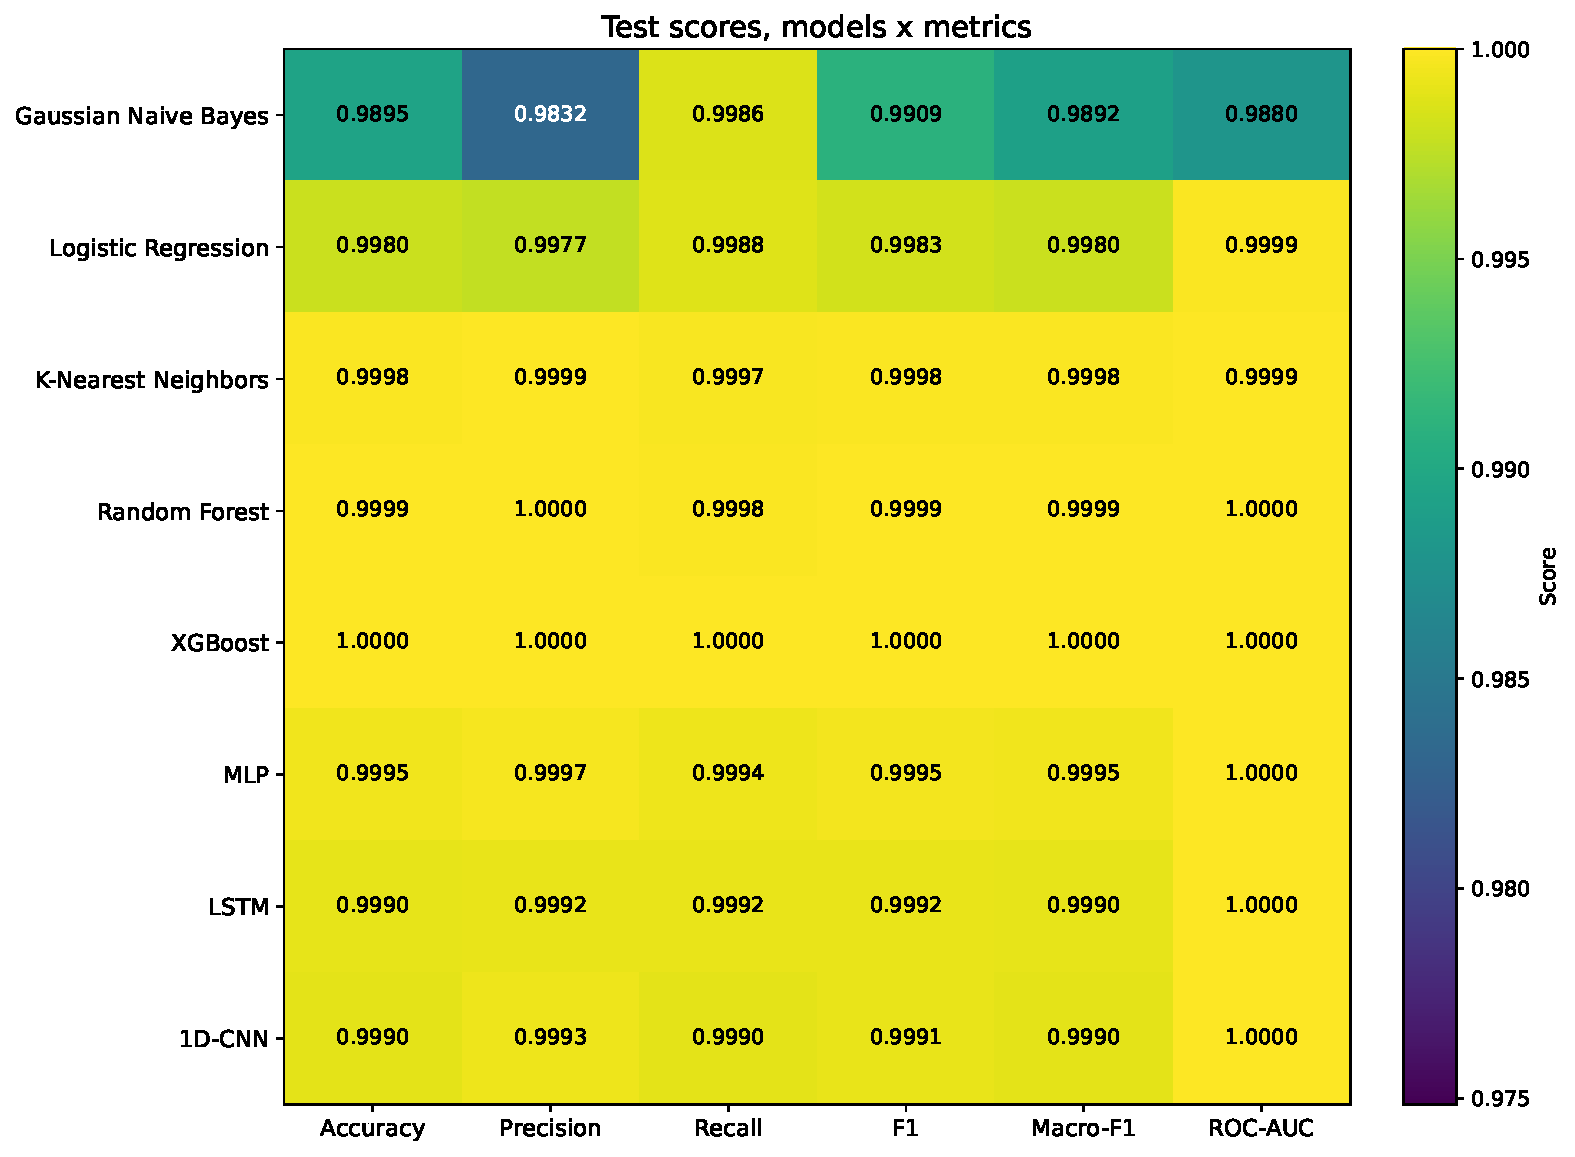
\includegraphics[width=0.75\textwidth]{metrics_heatmap.pdf}
\caption{Heatmap of the six test scores per model. Only Gaussian Naive Bayes (Precision 0.9832) and, less so, Logistic Regression are visibly different from the rest.}\label{fig:heat}
\end{figure}

\section{Errors instead of scores}
Accuracy alone is not informative here, since all models lie between 0.9895 and 1.0000, so we compare the number of errors (Figure~\ref{fig:errors}). XGBoost makes no error. Random Forest makes only 3 false negatives, KNN 1 false positive and 5 false negatives. The three neural networks make 18 (MLP), 32 (LSTM) and 33 (1D-CNN) errors, Logistic Regression 67 and Gaussian Naive Bayes 353, of which 327 are false positives. Gaussian Naive Bayes thus misses few attacks (Recall 0.9986) but raises many false alarms, which lowers its Precision to 0.9832. The LSTM is the only model with equally many FP and FN.

\begin{figure}[htb]
\centering
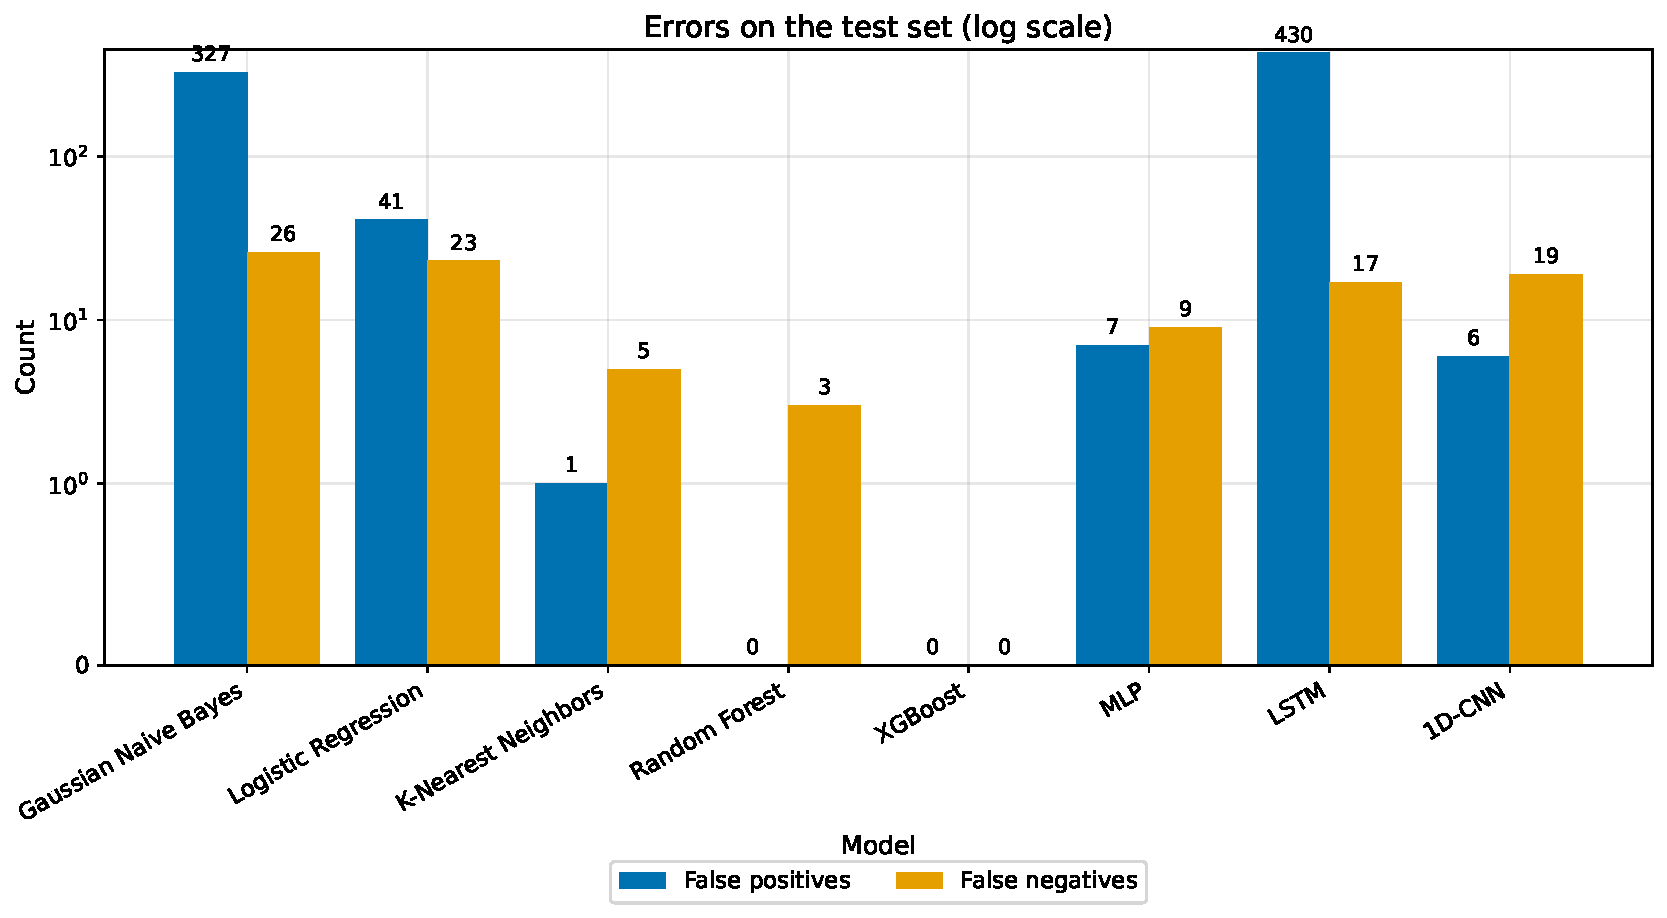
\includegraphics[width=0.85\textwidth]{errors_bar.pdf}
\caption{False positives and false negatives per model on the test set (log scale).}\label{fig:errors}
\end{figure}

Figure~\ref{fig:conf} shows the same information as row-normalised confusion matrices. On this scale only Gaussian Naive Bayes (0.0229 of the benign flows misclassified) and Logistic Regression (0.0031) differ visibly from the diagonal.

\begin{figure}[htb]
\centering
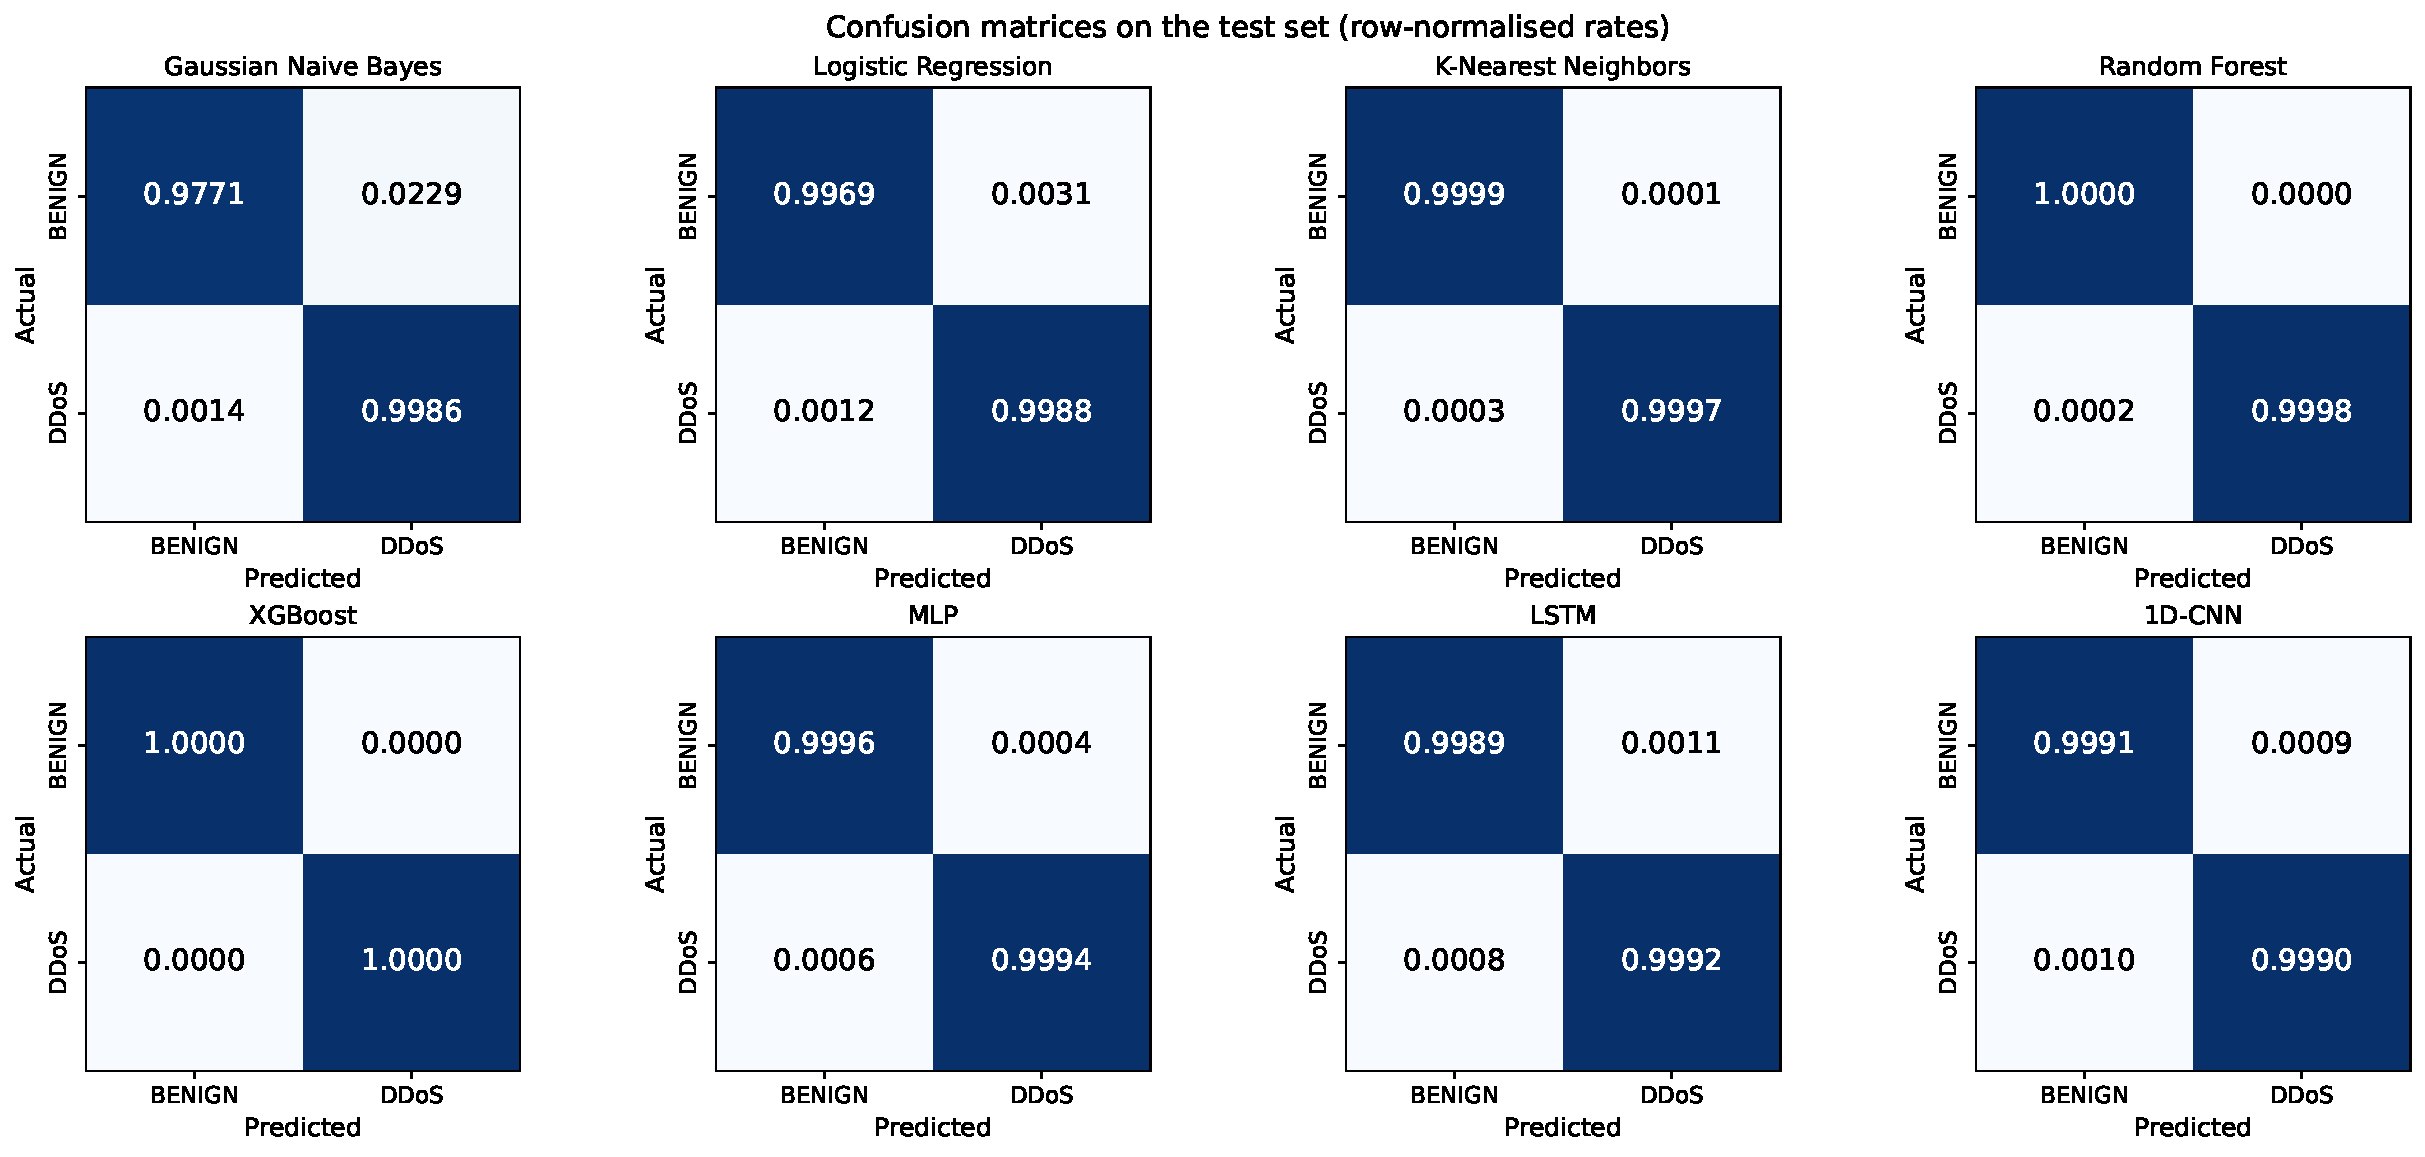
\includegraphics[width=\textwidth]{confusion_grid_normalized.pdf}
\caption{Row-normalised confusion matrices on the test set (rates with four decimals).}\label{fig:conf}
\end{figure}

\section{ROC curves}
The ROC-AUC values are 1.0000 for Random Forest, XGBoost, MLP, LSTM and 1D-CNN, 0.9999 for Logistic Regression and KNN and 0.9880 for Gaussian Naive Bayes. A plain ROC plot would show eight curves hugging the top-left corner, so we show two zoomed versions. Figure~\ref{fig:roczoom} zooms on false-positive rates up to 0.01 and true-positive rates from 0.990. The curves of XGBoost, Random Forest and KNN lie at the top. Among the others, the dashed curves of the neural networks stay above Logistic Regression, whose true-positive rate stays near 0.999 over this range. Gaussian Naive Bayes lies outside the view. Figure~\ref{fig:roclog} uses a logarithmic false-positive axis, which stresses the low false-alarm region that matters for a detector, with FPR $=0$ clipped at $10^{-5}$ (one false positive on the test set is about $7\cdot10^{-5}$). XGBoost, Random Forest and KNN reach a true-positive rate near 1 at the smallest false-positive rates, while Gaussian Naive Bayes needs a false-positive rate of about 0.02 to reach it. The KNN curve has only a few distinct points because its scores take only six values.

\begin{figure}[htb]
\centering
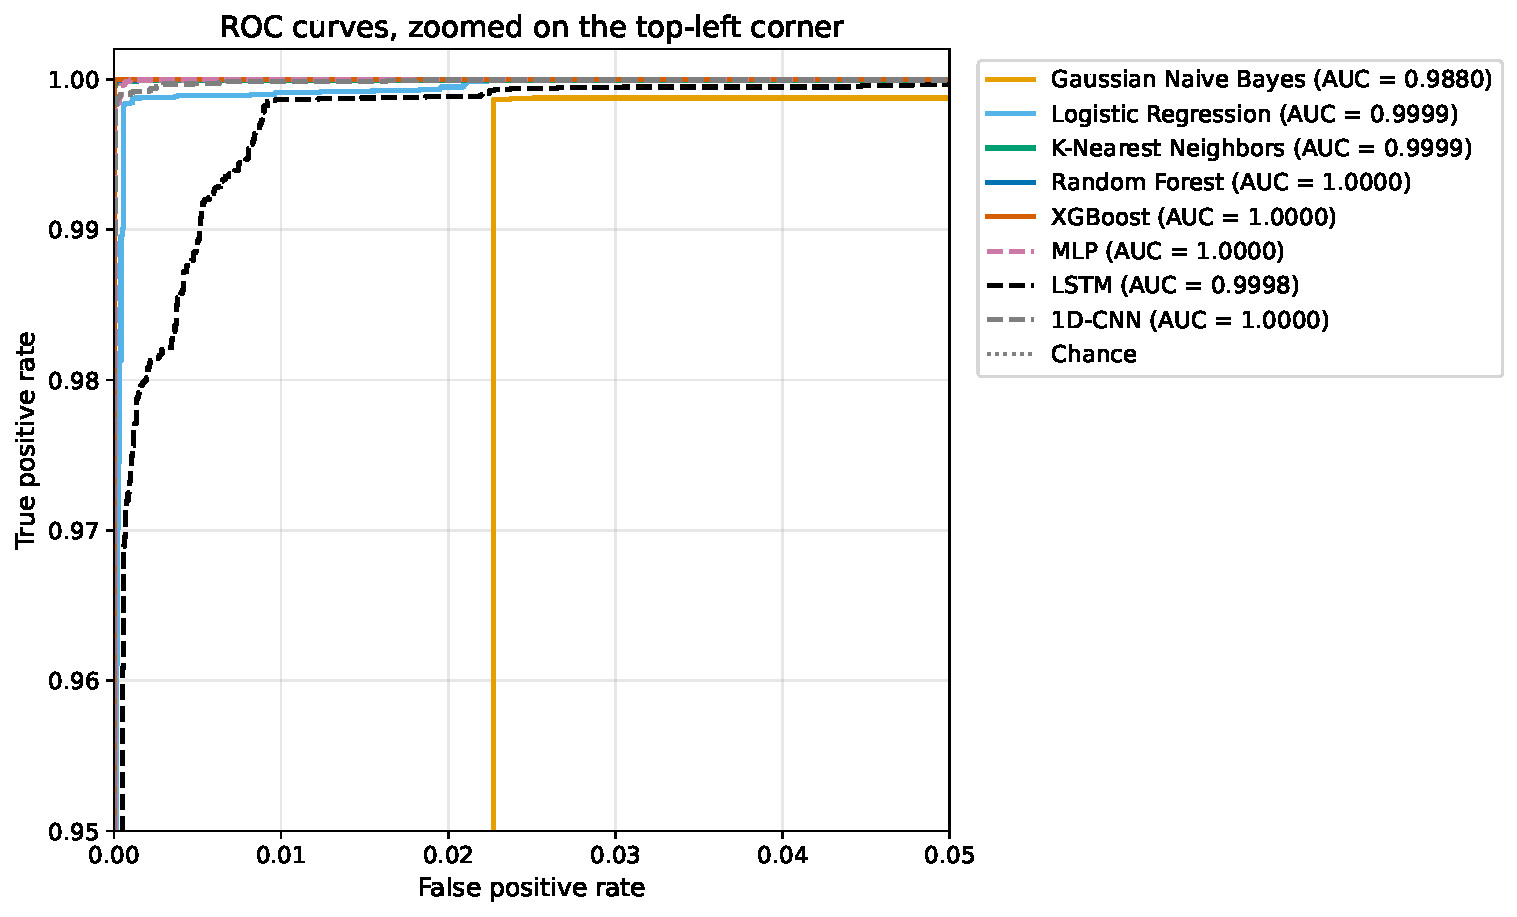
\includegraphics[width=0.85\textwidth]{roc_test_zoom.pdf}
\caption{ROC curves zoomed on the top-left corner (solid: ML models, dashed: neural networks). AUC values are given in the legend.}\label{fig:roczoom}
\end{figure}

\begin{figure}[htb]
\centering
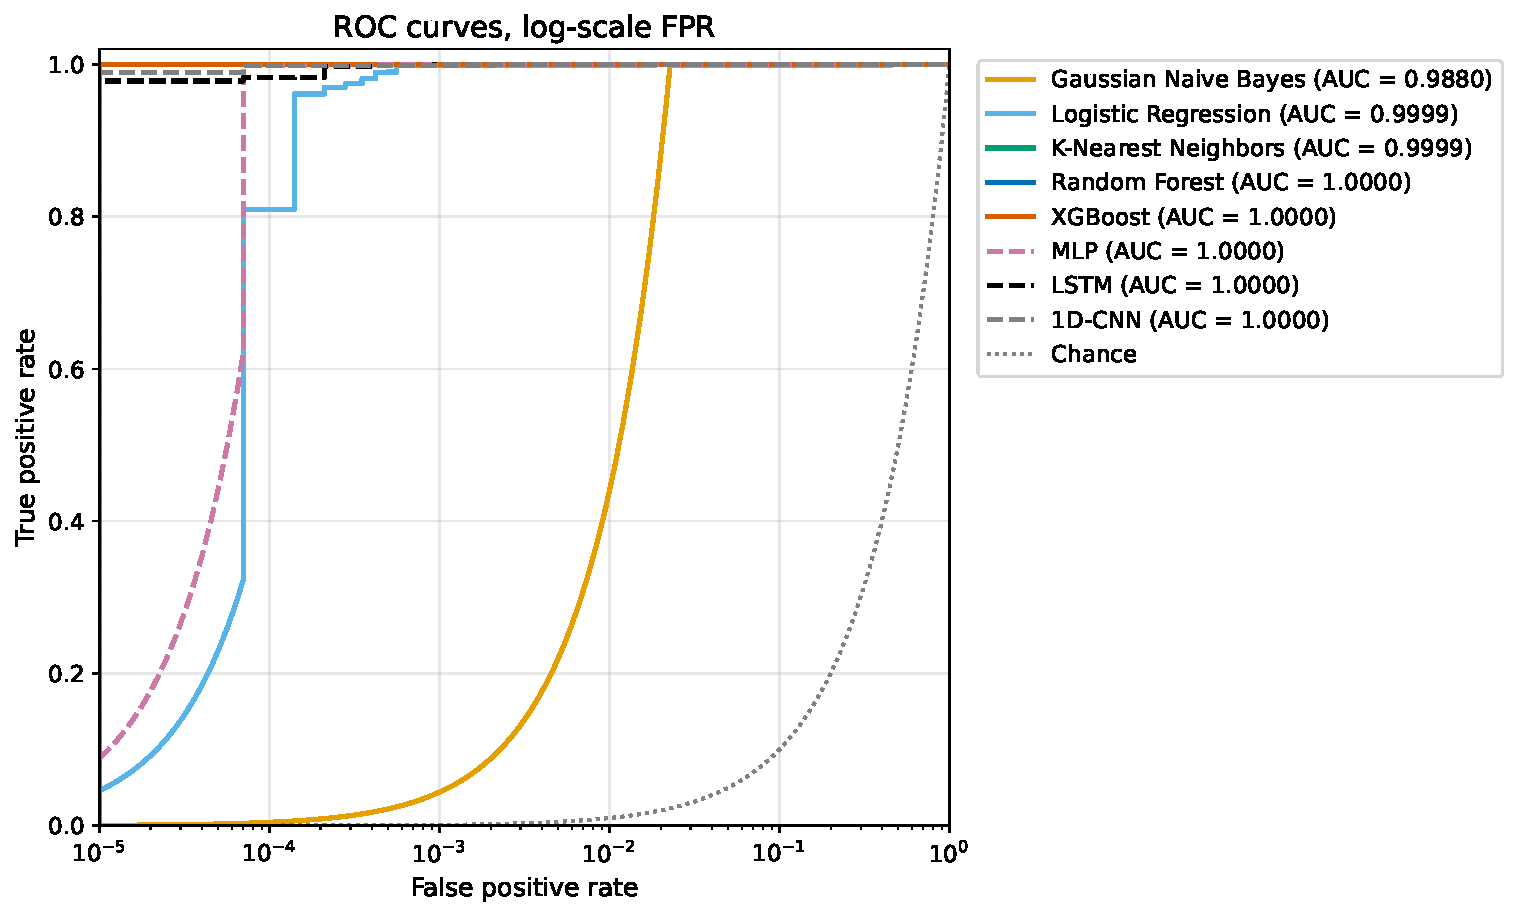
\includegraphics[width=0.85\textwidth]{roc_test_logx.pdf}
\caption{ROC curves with a logarithmic false-positive-rate axis; the dotted line is chance. Curves that start at the left edge and rise along a curved line (e.g.\ MLP, Logistic Regression) show the linear interpolation from FPR 0 to the first false positive drawn on a log axis, not poor performance at low FPR.}\label{fig:roclog}
\end{figure}

\section{Cost}\label{sec:cost}
Figure~\ref{fig:time} shows training and prediction times. Training is fastest for Gaussian Naive Bayes (0.063\,s) and KNN (0.008\,s, since it only stores the data), then XGBoost (2.021\,s) and Random Forest (3.847\,s); Logistic Regression takes 17.348\,s. The neural networks are the most expensive to train: MLP 42.244\,s, 1D-CNN 65.544\,s and LSTM 136.034\,s. KNN reverses the picture at prediction time: 4.204\,s for the test set, against at most 0.173\,s for every other model. That is the relevant cost for a detector that has to decide quickly. These times come from a single run and show the order of magnitude only.

\begin{figure}[htb]
\centering
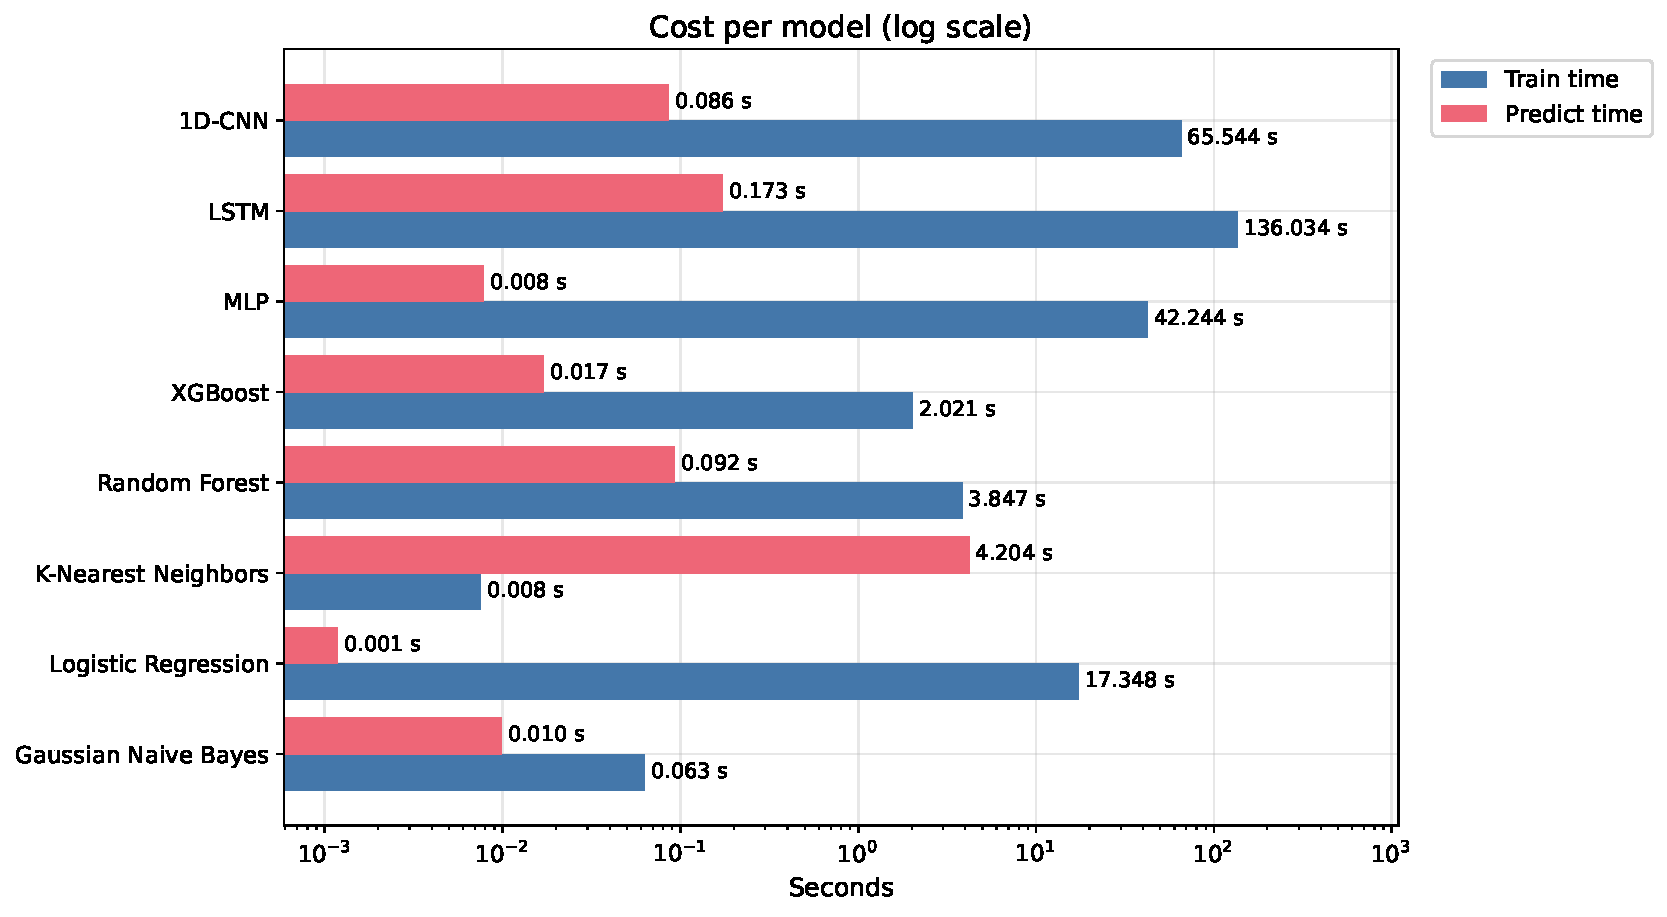
\includegraphics[width=0.85\textwidth]{time_bar.pdf}
\caption{Training and prediction time per model (log scale).}\label{fig:time}
\end{figure}

\section{Validation results}
Table~\ref{tab:val} gives selected scores on the validation set. The ranking is the same as on the test set, except that the 1D-CNN and the LSTM swap places and Random Forest ties with XGBoost (one false negative each). For XGBoost and the three neural networks, which use the validation set for early stopping, the validation scores are optimistic by construction, so the test scores are the figures to trust.

\begin{table}[htb]
\centering
\caption{Selected validation scores (33,462 flows), sorted by F1.}\label{tab:val}
\begin{tabular}{lrrrrr}
\toprule
Model & Accuracy & F1 & ROC-AUC & FP & FN \\
\midrule
Random Forest & 1.0000 & 1.0000 & 1.0000 & 0 & 1 \\
XGBoost & 1.0000 & 1.0000 & 1.0000 & 0 & 1 \\
K-Nearest Neighbors & 0.9997 & 0.9997 & 0.9999 & 3 & 7 \\
MLP & 0.9995 & 0.9996 & 1.0000 & 6 & 11 \\
1D-CNN & 0.9991 & 0.9992 & 0.9999 & 13 & 17 \\
LSTM & 0.9989 & 0.9990 & 0.9998 & 20 & 18 \\
Logistic Regression & 0.9982 & 0.9985 & 0.9998 & 42 & 17 \\
Gaussian Naive Bayes & 0.9890 & 0.9905 & 0.9875 & 349 & 18 \\
\bottomrule
\end{tabular}
\end{table}
